% Block scheme v5: the augmented-state row gets its own summer.
%
% v4 and everything before it draw the added-state row with EXACTLY ONE arrow entering it,
% g_aug, and the physical rows with a summer each. That asymmetry is the failure: g_aug is
% exactly zero at initialisation (baseline equality), so xbar is zero at every sample, the
% network reads zeros on those columns, and h_aug = 0 means nothing else can see xbar either.
% Measured consequence: ablation 1.0002x, improvement fraction F = 0.0007.
%
% v5 changes ONE region of the figure and nothing else. The xbar row now has a summer, like
% the physical rows always did, and three signals arrive at it:
%
%     xbar[k+1] = A_aa xbar[k] + B_z z[k] + g_aug(xhat[k], u[k])
%
%   A_aa   identified-pole recurrence, reads xbar off the state bus. Supplies MEMORY.
%          It is trainable in arms ii/iii and frozen only in the explicit frozen-pole control.
%   B_z    random input map, reads xtilde and u, NOT xbar (those columns are masked to zero,
%          so the block is drawn without an xbar input on purpose). Supplies DRIVE.
%   g_aug  unchanged from v4, still exactly zero at initialisation.
%
% In arms ii/iii both A_aa and B_z are trainable. The point is that their effective linear route
% is NON-ZERO before training starts,
% which is what makes the states exist at all. Measured: the poles receive gradient and still
% move under 0.5 Hz over 1044 updates, so placement decides the outcome.
%
% Everything else (state bus, setpoint bus, encoder, delay, router S, the three physical
% summers, h_aug = 0) is byte-identical to v4, so v4 and v5 can be shown back to back and the
% difference IS the argument.
%
% NEWMARK toggles the highlight colour on the three additions. Set it to black for the thesis
% figure and leave it blue for the slide, where the diff is the point.
%
% Compile: pdflatex jan-blockscheme-v5.tex
\documentclass[border=12pt]{standalone}
\usepackage{tikz}
\usetikzlibrary{arrows.meta, calc}
\usepackage{amsmath}
\usepackage{xcolor}

\definecolor{newmark}{RGB}{20,90,180}   % set to black for a plain thesis figure

\begin{document}
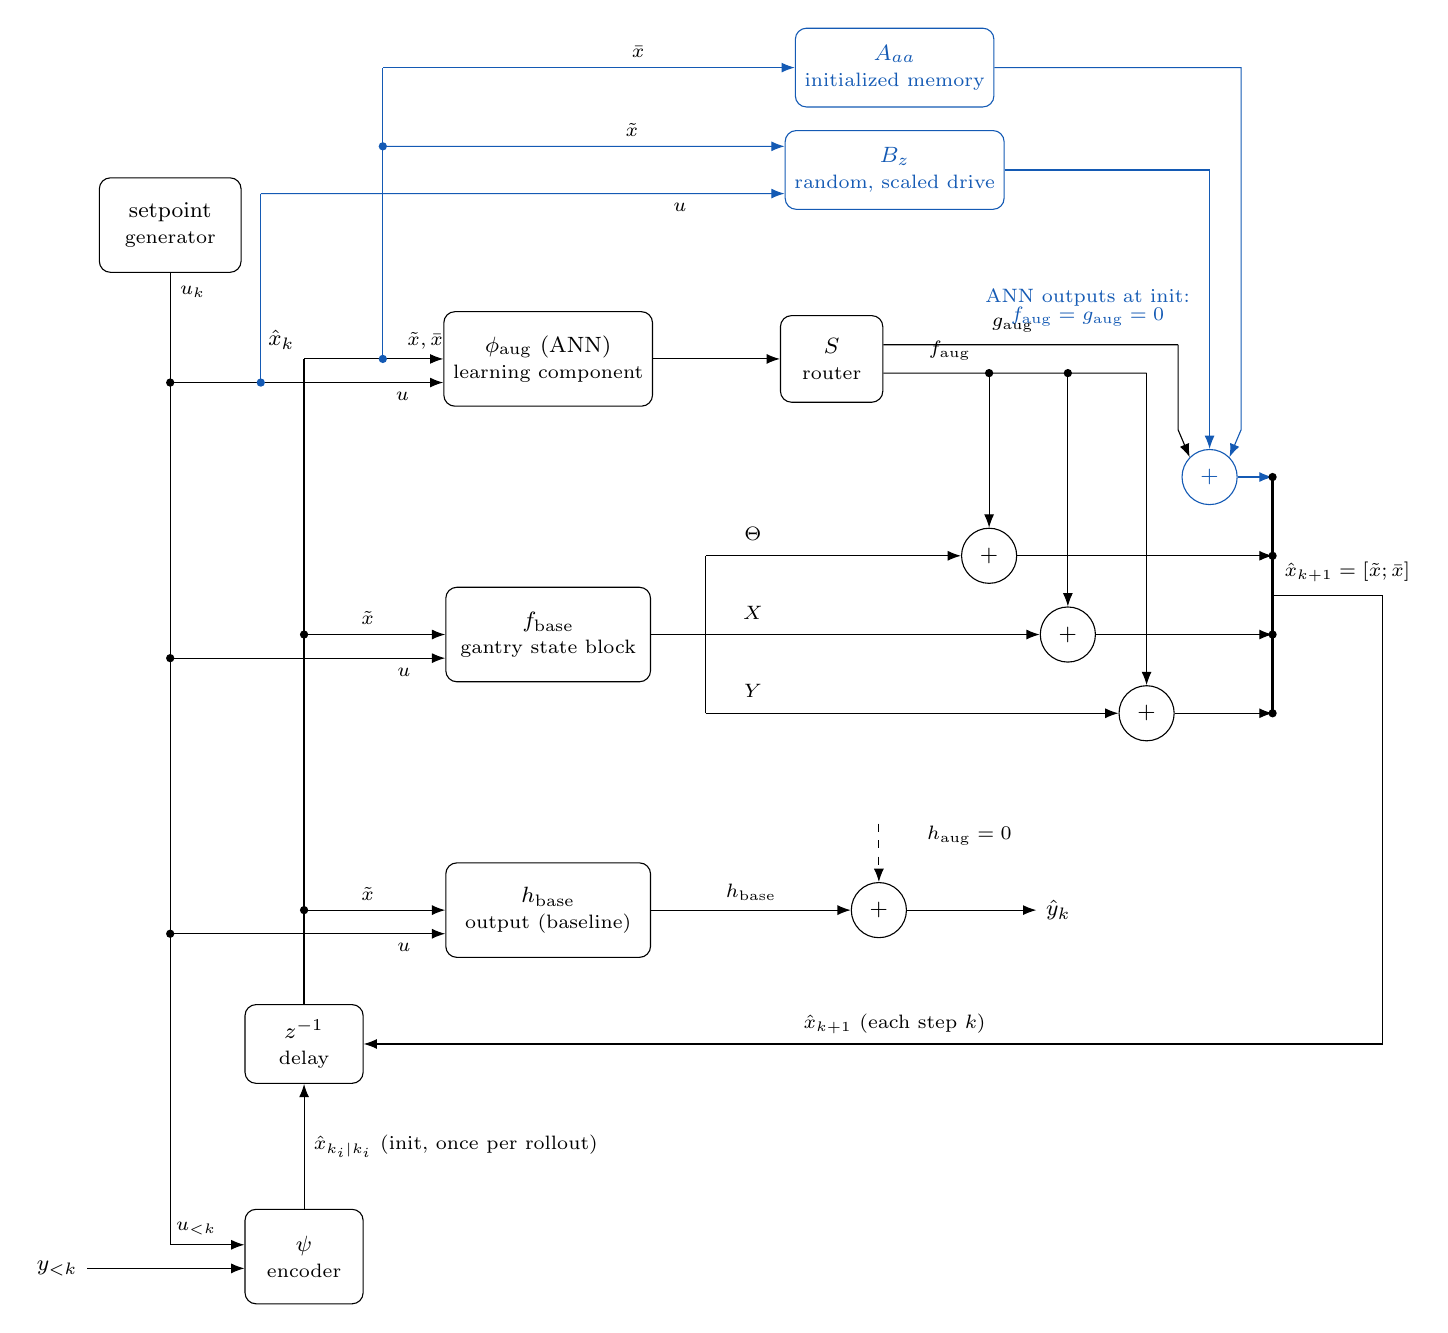
\begin{tikzpicture}[>=Latex, font=\footnotesize,
  block/.style={draw, rounded corners, minimum width=26mm, minimum height=12mm, align=center},
  rblock/.style={draw, rounded corners, minimum width=13mm, minimum height=11mm, align=center},
  small/.style={draw, rounded corners, minimum width=15mm, minimum height=10mm, align=center},
  sum/.style={draw, circle, minimum size=7mm, inner sep=0pt},
  jn/.style={circle, fill, minimum size=3pt, inner sep=0pt},
  nblock/.style={draw=newmark, text=newmark, rounded corners, minimum width=15mm,
                 minimum height=10mm, align=center},
  nsum/.style={draw=newmark, text=newmark, circle, minimum size=7mm, inner sep=0pt},
  nline/.style={draw=newmark},
  njn/.style={circle, fill=newmark, minimum size=3pt, inner sep=0pt}]

% ===== blocks =====
\node[block]  (ann)   at (-4.2, 3.5)  {$\phi_{\mathrm{aug}}$ (ANN)\\{\scriptsize learning component}};
\node[block]  (fbase) at (-4.2, 0)    {$f_{\mathrm{base}}$\\{\scriptsize gantry state block}};
\node[block]  (hbase) at (-4.2,-3.5)  {$h_{\mathrm{base}}$\\{\scriptsize output (baseline)}};
\node[rblock] (S)     at (-0.6, 3.5)  {$S$\\{\scriptsize router}};
\node[block, minimum width=18mm] (ref) at (-9.0, 5.2) {setpoint\\{\scriptsize generator}};

% ===== NEW: the augmented-state dynamics =====
\node[nblock] (Aaa) at (0.2, 7.2) {$A_{aa}$\\{\scriptsize initialized memory}};
\node[nblock] (Bz)  at (0.2, 5.9) {$B_z$\\{\scriptsize random, scaled drive}};

% ===== state bus (fed from the register/delay output) =====
\draw[thick] (-7.3,-4.7) -- (-7.3,3.5);
\node[above left=0pt] at (-7.3,3.5) {$\hat{x}_k$};
% label moved to pos 0.85 (v4 had 0.58) so it clears the new riser tap at x = -6.3
\draw[->] (-7.3,3.5) -- (ann.west)   node[pos=0.87,above]{\scriptsize $\tilde{x},\bar{x}$};
\draw[->] (-7.3,0)   -- (fbase.west) node[pos=0.45,above]{\scriptsize $\tilde{x}$};
\draw[->] (-7.3,-3.5)-- (hbase.west) node[pos=0.45,above]{\scriptsize $\tilde{x}$};
\node[jn] at (-7.3,0) {};
\node[jn] at (-7.3,-3.5) {};

% ===== setpoint bus: exogenous input u_k, generated (not fed back from data/state) =====
\draw[-] (ref.south) -- (-9.0,-7.75);
\node[right] at (-9.0,4.35) {\scriptsize $u_k$};
\draw[->] (-9.0,3.2)  -- ($(ann.west)+(0,-0.3)$)   node[pos=0.85,below]{\scriptsize $u$};
\draw[->] (-9.0,-0.3) -- ($(fbase.west)+(0,-0.3)$) node[pos=0.85,below]{\scriptsize $u$};
\draw[->] (-9.0,-3.8) -- ($(hbase.west)+(0,-0.3)$) node[pos=0.85,below]{\scriptsize $u$};
\node[jn] at (-9.0,3.2) {};
\node[jn] at (-9.0,-0.3) {};
\node[jn] at (-9.0,-3.8) {};

% ===== NEW: risers to A_aa and B_z, tapped off the SAME lines that already feed phi_aug =====
% A_aa reads xbar; B_z reads xtilde and u only, because its xbar columns are masked to zero.
\node[njn] at (-6.3,3.5) {};
\draw[nline] (-6.3,3.5) -- (-6.3,7.2);
\draw[nline,->] (-6.3,7.2) -- (Aaa.west) node[pos=0.62,above]{\scriptsize $\bar{x}$};
\node[njn] at (-6.3,6.2) {};
\draw[nline,->] (-6.3,6.2) -- ($(Bz.west)+(0,0.3)$) node[pos=0.62,above]{\scriptsize $\tilde{x}$};
% riser at x = -7.85, clear of the setpoint-generator box (its right edge is at x = -8.1)
\node[njn] at (-7.85,3.2) {};
\draw[nline] (-7.85,3.2) -- (-7.85,5.6);
\draw[nline,->] (-7.85,5.6) -- ($(Bz.west)+(0,-0.3)$) node[pos=0.80,below]{\scriptsize $u$};

% ===== router: f_aug trunk fans into Theta, X, Y; g_aug into the xbar summer =====
\draw[->] (ann.east) -- (S.west);
\node[sum] (tsum) at (1.4, 1.0) {$+$};
\node[sum] (xsum) at (2.4, 0)   {$+$};
\node[sum] (ysum) at (3.4,-1.0) {$+$};
% f_aug leaves S lower-right, runs as a trunk, drops once per physical channel
\draw[-]  ($(S.east)+(0,-0.18)$) -- (3.4,3.32);
\node[jn] at (1.4,3.32) {}; \node[jn] at (2.4,3.32) {};
\draw[->] (1.4,3.32) -- (tsum.north);
\draw[->] (2.4,3.32) -- (xsum.north);
\draw[->] (3.4,3.32) -- (ysum.north);
\node[above] at (0.9,3.36) {\scriptsize $f_{\mathrm{aug}}$};

% ===== NEW: the xbar summer, the one structural change =====
\node[nsum] (bsum) at (4.2, 2.0) {$+$};
% g_aug now arrives at the summer instead of dropping straight onto the bus-bar
\draw[-]  ($(S.east)+(0,0.18)$) -- (3.8,3.68);
\draw[->] (3.8,3.68) -- (3.8,2.6) -- (bsum.135);
\node[above] at (1.7,3.72) {\scriptsize $g_{\mathrm{aug}}$};
\node[newmark, align=center] at (2.65,4.15)
  {\scriptsize ANN outputs at init:\\[-1mm]\scriptsize $f_{\mathrm{aug}}=g_{\mathrm{aug}}=0$};
% B_z and A_aa arrive at the same summer
\draw[nline,->] (Bz.east)  -- (4.2,5.9) -- (4.2,2.6) -- (bsum.north);
\draw[nline,->] (Aaa.east) -- (4.6,7.2) -- (4.6,2.6) -- (bsum.45);
\draw[nline,->] (bsum.east) -- (5.0,2.0);

% ===== f_base fan: every physical channel now passes through its own summer =====
\draw[-]  (-2.2,-1.0) -- (-2.2,1.0);               % fan bar
\draw[->] (-2.2,1.0)  -- (tsum.west);
\draw[->] (tsum.east) -- (5.0,1.0);
\node at (-1.6, 1.28) {\scriptsize $\Theta$};
\draw[->] (fbase.east) -- (xsum.west);             % X line, aligned with f_base
\draw[->] (xsum.east)  -- (5.0,0);
\node at (-1.6, 0.28) {\scriptsize $X$};
\draw[->] (-2.2,-1.0) -- (ysum.west);
\draw[->] (ysum.east) -- (5.0,-1.0);
\node at (-1.6,-0.72) {\scriptsize $Y$};

% ===== bundle: concatenation bus-bar (NOT a sum) =====
\draw[line width=1.3pt] (5.0,-1.0) -- (5.0,2.0);
\node[jn] at (5.0,2.0) {}; \node[jn] at (5.0,1.0) {};
\node[jn] at (5.0,0) {}; \node[jn] at (5.0,-1.0) {};
\draw[-] (5.0,0.5) -- (6.4,0.5);
\node[above] at (5.95,0.55) {\scriptsize $\hat{x}_{k+1}=[\tilde{x};\bar{x}]$};

% ===== state register z^-1 at the base of the bus; encoder sets its initial condition =====
\node[small] (delay) at (-7.3,-5.2) {$z^{-1}$\\{\scriptsize delay}};
% running input: the next state, fed back from the right (each step)
\draw[-]  (6.4,0.5) -- (6.4,-5.2);
\draw[->] (6.4,-5.2) -- (delay.east);
\node at (0.2,-4.95) {\scriptsize $\hat{x}_{k+1}$ (each step $k$)};
% encoder below, feeding the initial-condition (bottom) port -- fires once per rollout
\node[block, minimum width=15mm] (enc) at (-7.3,-7.9) {$\psi$\\{\scriptsize encoder}};
% u history taps the setpoint bus; y history comes from the measured data
\draw[->] (-9.0,-7.75) -- ($(enc.west)+(0,0.15)$) node[pos=0.35,above]{\scriptsize $u_{<k}$};
\draw[<-] ($(enc.west)+(0,-0.15)$) -- ++(-2.0,0) node[left]{$y_{<k}$};
\draw[->] (enc.north) -- (delay.south) node[pos=0.5,right]{\scriptsize $\hat{x}_{k_i|k_i}$ (init, once per rollout)};

% ===== output readout: yhat = h_base (+) h_aug, h_aug = 0 =====
\node[sum] (osum) at (0,-3.5) {$+$};
\draw[->] (hbase.east) -- (osum.west) node[pos=0.5,above]{\scriptsize $h_{\mathrm{base}}$};
\draw[->, dashed] (0,-2.4) -- (osum.north);
\node at (1.15,-2.55) {\scriptsize $h_{\mathrm{aug}}=0$};
\draw[->] (osum.east) -- (2.0,-3.5) node[right]{$\hat{y}_k$};

\end{tikzpicture}
\end{document}
